\documentclass[12pt, titlepage]{article}
\usepackage[a4paper, total={6.5in, 10in}]{geometry}
\usepackage{hyperref}
\usepackage{listings}
\usepackage{color}
\usepackage{float}
\usepackage{tocloft}

\cftsetindents{section}{0em}{2em}
\cftsetindents{subsection}{0em}{2em}

\renewcommand\cfttoctitlefont{\hfill\Large\bfseries}
\renewcommand\cftaftertoctitle{\hfill\mbox{}\vspace*{6mm}}

\setcounter{tocdepth}{2}

\definecolor{dkgreen}{rgb}{0,0.6,0}
\definecolor{gray}{rgb}{0.5,0.5,0.5}
\definecolor{mauve}{rgb}{0.58,0,0.82}

\lstset{frame=tb,
  language=Haskell,
  aboveskip=3mm,
  belowskip=3mm,
  showstringspaces=false,
  columns=flexible,
  basicstyle={\small\ttfamily},
  numbers=none,
  numberstyle=\tiny\color{gray},
  keywordstyle=\color{blue},
  commentstyle=\color{dkgreen},
  stringstyle=\color{mauve},
  breaklines=true,
  breakatwhitespace=true,
  tabsize=3
}

\usepackage{amsmath}
\usepackage{amssymb}
\usepackage{enumitem}
\usepackage{braket}
\usepackage{qcircuit}
\usepackage{graphicx}

\newcommand{\code}{CS-IS-2010-1}
\newcommand{\name}{Functional Programming Report}
\newcommand{\me}{Santripta Sharma}

\newcommand{\prob}[1]{\mathbb{P}\left[#1\right]}

\newcommand{\kz}{\ket{0}}
\newcommand{\ko}{\ket{1}}
\newcommand{\kp}{\ket{\phi}}
\newcommand{\ks}{\ket{\psi}}
\newcommand{\kso}{\ket{\psi_1}}
\newcommand{\kst}{\ket{\psi_2}}

\newcommand{\rec}[1]{\frac{1}{#1}}

\newtheorem{lemma}{Lemma}

\newenvironment*{qparts}{\begin{enumerate}[label=(\alph*)]}{\end{enumerate}}

\title{Inference \& Evaluation Engine for Feed-Forward Neural Networks in Haskell\vspace*{2mm}

{\large \code: \name}

{\large Supervisor: \href{https://www.ashoka.edu.in/profile/partha-pratim-das/}{Partha Pratim Das}}}
\author{\textbf{\me}\\(1020211136)}
\date{\today}

\markright{\code\hspace{0.5in}\name\hspace{0.5in}\me}

\parindent=0pt

\begin{document}
\maketitle

\tableofcontents
\newpage

\section{Acknowledgements}
I would like to thank Professor Partha Pratim Das for instructing this Independent Study Module, and allowing us to explore the expressive field of functional programming. Additionally, I would like to thank my peers also taking this course for cultivating a constructive learning environment for this course.
\newpage

\section{Introduction}
Through the course of this project, we have developed a command-line tool to run inference on (or evaluate) an arbitrary feed-forward neural network (for classification tasks). The primary goal for the project was to gain familiarity with haskell (and the functional programming paradigm) by implementing a medium-sized project using it.\bigskip

In this regard, the project has been quite succesful, forcing me to cover a lot of the bases in a relatively short time. The entire process took me from the basics, performing command-line I/O, and using the haskell tool stack, all the way to writing parser combinators for binary data, using monads, and implementing test suites with HSpec.\bigskip

Besides the learning outcomes from the project, the tool that has been developed is also useful in practical settings. It has been designed \& developed keeping in mind optimality, generalizability, and usability. An example use case of this tool is one where the user has been handed a trained classifier network (by, say, a tech-consultancy firm), and they wish to verify its performance on their data, without writing an evaluation/inference script on their own (due to time constraints or inexperience with the technology).

\section{Background \& Motivation}
\subsection{Motivation}\label{sec:3.1}
Today, Machine Learning has left no domain untouched. What initially started as a niche subfield of statistics has now found its application in nearly every sector \& discipline. This poses a simple problem: A large chunk of the users of these models are not familiar with how they work or how to use them. This has led to widespread black-boxing, where the development/training of the model is often outsourced to someone with this technical knowledge, with the 'client' being given instructions on how to use the model.\bigskip

Besides the inherent security risk, where the external party could place a backdoor into the model, this approach also forces the client to take the external party at their word when it comes to the effectiveness of the model, at least initially, which opens the door up to being defrauded. Additionally, in some cases, the instructions provided may be obtuse, rendering the client unable to use the model.\bigskip

Therefore, there is a need to be served for providing a solution that can perform inference and evaluation on these models, while also being friendly to users who aren't very tech-savvy. In this project, we particularly focus on a popular subclass of ML models, the feed-forward classifier, which is a generalisation of linear/logistic regression, and a foundational piece in most deep neural networks, with this unique position leading it to be one of the most common architectures for these models.

\subsection{Background: Feed-Forward Networks} \label{sec:3.2}
\begin{figure}
	\includegraphics[width=0.8\pdfpagewidth]{../images/FFN-structure.png}
	\caption{\label{fig:1}a generic FFN with $n_{hidden} = 2$}
\end{figure}
The Feed-Forward Network (FFN) is a versatile network architecture for deep neural networks, able to be used as both classifiers or regressors (though this project restricts its scope to the former). It is comprised of a set of layers ($L = \{L_1, L_2, \dots, L_{n_{hidden} + 2}\}$), each containing nodes, called 'neurons', each of which are connected to every neuron in the next layer by weighted edges. Each neuron also has an associated 'activation' value, though this is only meaningful while the model is being inferenced. Figure \ref{fig:1} provides a pictorial representation of this architecture. There are three types of layers in the networks:
\begin{itemize}
	\item \textbf{Input Layer} ($L_1$): The first layer of the network is the input layer. Here, each neuron's activation value corresponds directly to the value of a distinct feature in the datapoint currently being inferenced. From this, we derive the relation:
	\begin{flalign}
		|L_1| = in\_dim
	\end{flalign}
	Where $in\_dim$ is the dimensionality (number of features) of a datapoint in our dataset.

	\item \textbf{Hidden Layers} ($L_2, \dots, L_{n_{hidden} + 1}$): The layers between the first and last (exclusive) are the hidden layers. \textbf{The model's architecture is parametrised by the number of hidden layers ($n_{hidden}$), and the size of each hidden layer (the number of neurons in it)}, which can both be any integer (though these are usually selected very carefully depending on the problem). On each of these layers, a non-linear activation function is applied after activations are calculated, allowing the network to capture non-linear relations (eg. ReLU).
	
	\item \textbf{Output Layer} ($L_{n_{hidden + 2}}$): The final layer of the network is the output layer. Here, each neuron's activation values correspond (through some function) to the likelihood that the datapoint currently being inferenced belongs to a distinct class. This unknown function is called a non-linear activation function, and \textbf{is another parameter in the model's architecture}, with the softmax function being most commonly applied to classification tasks. We also have the relation:
	\begin{flalign}
		|L_{n_{hidden + 2}}| = out\_dim
	\end{flalign}
	Where $out\_dim$ is the number of distinct classes our datapoint can belong to.
\end{itemize}
While the model architecture is parametrised by the number of hidden layers, size of each hidden layer, and the choice of activation function to be applied at the output layer, being a machine learning architecture, it also contains a large number of trainable parameters. We omit discussion of the training procedure, due to it being out of scope for this project.\bigskip

The output of the training are the trainable parameters, the weights \& biases. As mentioned earlier, $\forall i > 1$, each neuron in $L_i$ is connected to each neuron in the layer $L_{i-1}$ by a weighted edge. Then, the weights matrix for this layer is simply a submatrix of the adjacency matrix representation of the subgraph induced by these adjoining edges (if we discard the matrix elements corresponding to nodes not joined by an edge, i.e., nodes in the same layer). Then, if $|L_i| = n_i, |L_{i - 1}| = n_{i - 1}$, the weights matrix for this layer $W_i: n_i \times n_{i - 1}$. The propagation formula for the FFN at this layer is given by:
\begin{flalign}
	X_i = \text{Activation}(W_iX_{i - 1} + B_i\label{eq:3})
\end{flalign}
Where $X_i, X_{i - 1}$ are the neuron activations at layers $i, (i - 1)$ respectively (these are column vectors, so $X_i: n_i \times 1, X_{i - 1}: n_{i - 1} \times 1$), $B_i: n_i \times 1$ is the bias column vector for this layer (trained parameter), and Activation($\cdot$) is the non-linear activation function (preserves matrix dimension). The knowledge that activation vectors ($X_i$s) are represented as column vectors, along with an understanding of matrix multiplication can be used to derive the following lemmas:
\begin{lemma} \label{lem:1}
	Given the weights matrix $W_i: a \times b$ at layer $L_i$, we have that $n_{i - 1} = b$.
\end{lemma} \label{lem:2}
\begin{lemma}
	Given the weights matrix $W_i: a \times b$ at layer $L_i$, we have that $n_i = a$.
\end{lemma}
Similarly, using our knowledge of matrix-matrix addition, we have:
\begin{lemma} \label{lem:3}
	Given the weights matrix $W_i: a \times b$ at layer $L_i$, the biases vector $B_i$ has the shape $B_i: a \times 1$.
\end{lemma}

\section{Literature Survey}
\subsection{Existing Neural Network Libraries}
Before we implement custom logic for reconstructing and running inference on a FFN, we first check the Haskell ecosystem for any existing neural network/machine learning libraries.\bigskip

We immediately found \href{https://hackage.haskell.org/package/neural}{neural}, a pure haskell framework for training and inferencing on various kinds of neural networks. Additionally, we find \href{https://github.com/HuwCampbell/grenade}{grenade}, \href{https://hackage.haskell.org/package/neural-network-hmatrix}{neural-network-hmatrix}, and \href{https://hackage.haskell.org/package/hnn}{hnn}. Unfortunately, all of them have the same problems.\bigskip

For our chosen problem, they are all overkill, attempting to provide a generic framework for training and using neural networks. The training part adds the majority of the overhead to the interfaces provided by these libraries, but we do not require any training support for this project. Adding to this, our project only cares about a very specific architecture, the FFN, whereas these projects pursue support for many architectures, leading to a less overall flexible (programmatic) interface for our case, compared to one we design on our own.\bigskip

For these reasons, we choose to implement the inference without the support of a deep learning library.

\subsection{Fast Linear Algebra in Haskell} \label{sec:4.2}
As seen in \eqref{eq:3}, the computation we perform during inference is essentially a series of matrix multiplications (and additions). In order to optimise this, our first task is to determine how haskell supports these operations.\bigskip

\begin{table}
	\centering \begin{tabular}{|c|c|c|c|}
		\hline \textbf{Library} & $n = 10$ & $n = 50$ & $n = 100$\\
		\hline DLA & 2.65us & 289.0us & 2.24ms\\
		\hline Hmatrix & 1.32us & 55.8us & 292.0us\\
		\hline NumHask & 714.0us & 63.5ms & 593.0ms\\
		\hline Massiv & 12.0us & 205.0us & 1.52ms\\
		\hline Massiv (Parallel) & 76.1us & 220.0us & 866.0us\\
		\hline Matrix & 12.6us & 1.1ms & 8.44ms\\
		\hline Naive C Implementation & 51us & 323us & 4.78ms\\
		\hline
	\end{tabular}
	\caption{\label{tab:1} \href{https://github.com/Magalame/fastest-matrices}{Linear Algebra Library Benchmark (matrix multiplication of size $n \times n$)}}
\end{table}
At a cursory glance, it can be seen that \href{https://wiki.haskell.org/Applications_and_libraries/Mathematics#Linear_algebra}{there are various linear algebra libraries available for use with haskell}. In order to hone down on one library for usage, \href{https://github.com/Magalame/fastest-matrices}{this benchmark from 2015} is the best evidence we have to go off (short of running our own benchmark). Table \ref{tab:1} displays their results for the matrix multiplication task.\bigskip

According to this benchmark, the \href{https://hackage.haskell.org/package/hmatrix}{Hmatrix} library achieves SOTA performance for both the matrix multiplication and repeated matrix multiplication task (in a single-threaded setup). Then, we choose to utilise this library for maximising performance.

\section{Problem Statement}
\subsection{Problem Statement}
Develop a classification model over the Iris Dataset and store the model. Then write a Haskell code to restore the model, input new data (based on the four features of the iris) and generate a prediction in real time.
\begin{enumerate}
	\item Input: The Iris Dataset.
	\item Output: Real-time prediction for the class of the flower of a new data row containing the sepal width, petal width, sepal length and petal length.
	\item Method: You can use Python to train and save a classification model (SVM or NN). However, restoring the model and the real-time prediction of a new data row has to be written only in Haskell.
\end{enumerate}

\subsection{Objectives}
Based on this problem statement \& initial motivation, we aim to develop a system which:
\begin{itemize}
	\item Should be able to load a trained classification model.
	\item Given any new data point of the same format as the iris dataset by the user, should be able to use the loaded model to make a prediction on this data and report it to the user.
	\item Should be as performant as possible, since the problem description suggests that the application domain is a real-time system.
	\item Should be simple to use for a layperson.
	\item Should generalise beyond the iris dataset.
\end{itemize}

\section{Scope}
In order to fulfill our objectives, we have developed a system with the following featureset:
\begin{enumerate}
	\item Parsing capabilities to restore the shape, weights, and biases of \textbf{an arbitrary} FFN classifier from a file.
	\item Interactive \& batched modes of performing inference. \begin{itemize}
		\item \textbf{Interactive}: The user enters a single new datapoint and gets predictions for it in real-time. Structured as a Read-Eval-Print-Loop (REPL).
		\item \textbf{Batched}: The user provides many datapoints in a csv file, and receives predictions for each point.
	\end{itemize}
	\item An evaluation mode: an extension of batched inference mode which also takes in expected outputs, and determines model accuracy.
\end{enumerate}
To expand on point 1, since the type of model (FFN) is known, we can generalise the system to work with any classifier following that architecture, since this is independent of the particular dataset used, as long as that dataset only contains numeric feature. This allows the system to be reused for similar tasks beyond the Iris dataset, providing us the generality we desire.\bigskip

However, we do limit the class of models we allow to using ReLU (at the hidden layers) \& Softmax (at the output layer) activations, which covers most, but not all, FFN classifiers.

\begin{figure}
	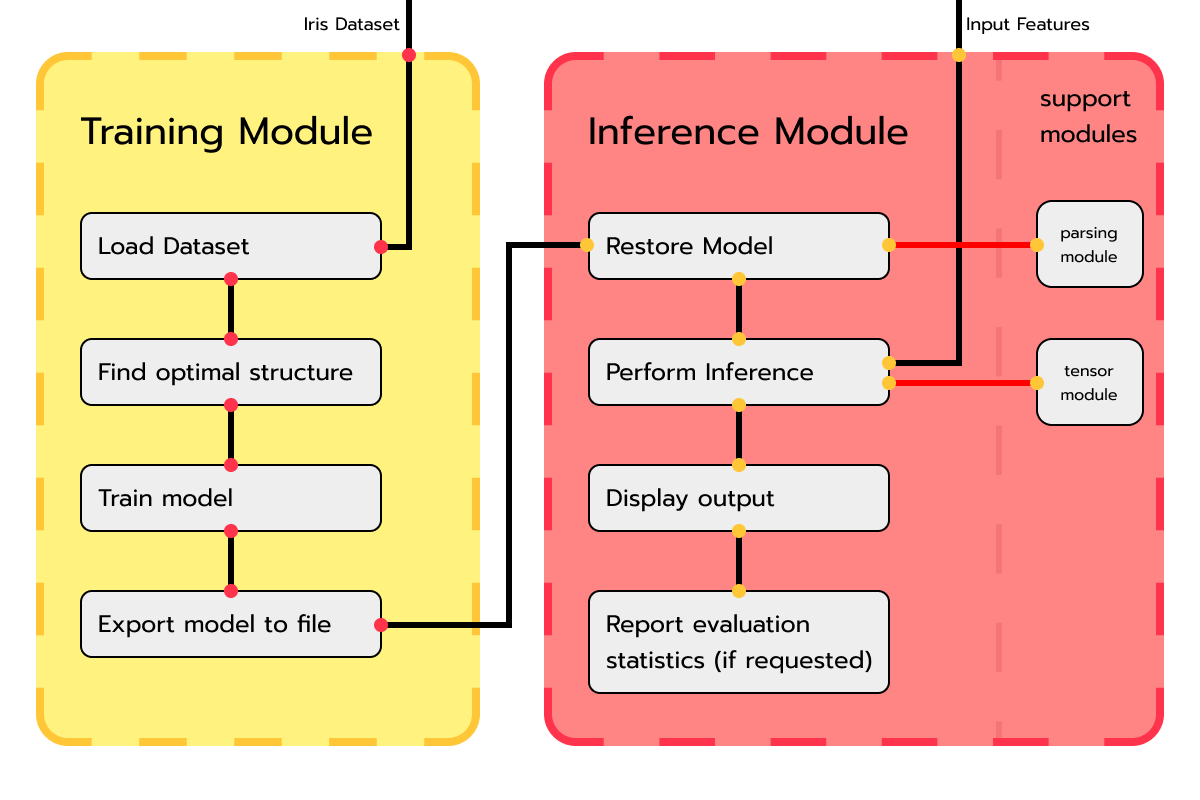
\includegraphics[width=0.85\pdfpagewidth]{../images/modules.png}
	\caption{\label{fig:2}the high-level design of the system}
\end{figure}

\section{Methodology \& Design}
\subsection{Architecture}
Since we are only concerned with running the inference for a new row for this dataset, we train our classification models separately (for testing purposes) before runtime. At runtime, we restore the structure, weights, and biases of the model, and push the given feature vector through the model in order to arrive at the inferred output.\bigskip

Then, the system can broadly be divided into two modules, the training module \& the inference module. These operate independently from each other, with the only interface between them being the inference module taking the training module's output (model structure, weights, biases) as its input, which is then used to reconstruct the model. Figure \ref{fig:2} illustrates the general flow of this architecture.

\subsection{Trained Model Format}
From Section \ref{sec:3.2}, we know that a feedforward neural network is comprised of several layers of neurons, with each layer (besides the input layer) having a matrix of weights \& a vector of biases associated with itself.\bigskip

Then, our naive model format is a binary file structured as follows:
\begin{verbatim}
number of layers
for each non-input layer in the network:
    weights matrix rows
    weights matrix columns
    weights matrix
    biases vector length
    biases vector
\end{verbatim}
Immediately, from lemma \ref{lem:3}, we can reduce this to a compacted format:
\begin{verbatim}
number of layers
for each non-input layer in the network:
    weights matrix rows
    weights matrix columns
    weights matrix
    biases vector
\end{verbatim}
We can make another space optimisation by noticing that lemma \ref{lem:1} allows us to infer the number of columns in the weights matrix of one layer from the number of neurons in the previous layer. Since the format is defined iteratively over layers, we can exploit this relation while parsing using memoisation. All we need to begin is the number of neurons in the input layer.
\begin{verbatim}
number of layers
number of neurons in input layer
for each non-input layer in the network:
    weights matrix rows
    weights matrix
    biases vector
\end{verbatim}
Since each stored integer here is 4 bytes wide, we have brought down the size of our format from $4\times (3l + 1) + D = 12l + D + 4$ bytes, where $l$ is the number of non-input layers and $D$ is the constant size of the actual data (weights \& biases) to $4\times(l + 2) + D = 4l + D + 8$ bytes, which scales much better with number of layers. Then, we have managed to enhance the information density of our format using our observations about the network architecture.

\subsection{Training Module}
The purpose of the training module is to provide us with a set of models we can use to test our inference module. As such, we don't strictly require a high performance model. However, we still perform some basic hyperparameter selection after loading the dataset in using a 5-fold cross validation approach to determine the shape of the network (number \& size of hidden layers).\bigskip

The model architecture used is the one mentioned above, a simple feedforward network, a sequence of linear layers using the ReLU activation function between the hidden layers, and the softmax activation at the end. Using a grid search, we find the top 5 performing shapes, and also one poorly performing shape, out of a generated set of possible shapes for the network.\bigskip

Before fitting 6 models using these shapes on the data, the data is transformed by converting the output classes column from textual labels to numerical labels, to avoid any ordering ambiguities arising during the training process. This transformed data is then split into training \& test sets, and we fit the models on the training set.\bigskip

Finally, we write the networks' weights and biases into model files, which can then be used by the inference module.

\subsection{Inference Module}
The inference module constitutes the bulk of the codebase. It produces an executable with the following signature:
\begin{verbatim}
inference-exe <path_to_model_file> [<path_to_batch_csv>] [<path_to_labels_csv>]
\end{verbatim}
If the second, optional argument is omitted, it starts in interactive mode. Otherwise, it starts in batched mode. If the third argument is provided, it runs in evaluation mode.\bigskip

In either case, its first task is to restore the model from the given model file. Here, we utilise the parsing support module, which is written using parser combinators. Further implementation details of the parser are discussed in the Test Plan \& Prototype Details section. \bigskip

Through this parsing process, the model shape, and its parameters are loaded into a data structure which takes the form of a list of layers, where each layer stores its input \& output shapes, and the weights \& biases matrices.\bigskip

Next, based on which mode it was started in, the system either enters a REPL or parses the input batch csv file it was provided (again, with the help of the parsing support module). In either mode, once the feature vector(s) are acquired, the tensor support module is used to perform the sequence of computations that lead to the final prediction.\bigskip

The final output (for each feature vector) is the predicted class and the probabilities associated with each class. If the program was started in evaluation mode, it will also report an accuracy metric, that is, how many of the predicted outputs matched their correct labels as given in the labels csv file, as a percentage.

\section{Work Done}
\subsection{Tooling}
\subsubsection{Training Module}
The training module is written in python, using numpy, pandas, and sklearn to perform the data processing \& model training/selection.\bigskip

\subsubsection{Inference Module}
The inference module is written in Haskell. We use the Haskell Tool Stack (or just Stack) as our build tool. The following dependencies are used:
\begin{itemize}
	\item \textbf{hmatrix}\\
	As described earlier in \ref{sec:4.2}, this library provides vector \& matrix types, along with the definitions for common mathematical operations on them, including matrix multiplication, conversions, etc.\bigskip

	It is the backbone of tensor support module, which is used to finally perform the inference once the inputs have been parsed.

	\item \textbf{\href{https://hackage.haskell.org/package/cereal}{cereal}}\\
	Cereal is a highly performant serialization library for binary data formats. We choose it over the alternatives due to its out of the box support for parsing IEEE754 double-precision floating point numbers from binary files, which the alternatives (like binary or attoparsec) do not support.\bigskip

	It is used by the parsing support module to parse our model files.

	\item \textbf{\href{https://hackage.haskell.org/package/cassava-0.5.3.1}{cassava}}\\
	Cassava is Haskell's most popular library for working with csv data, which we use to parse batch dataset \& groundtruth files.
\end{itemize}

\subsubsection{Testing/Miscellaneous}
A mix of bash \& python scripts is used to implement the end-to-end tests and certain convenient utilities (eg. infer.py for loading and making predictions using sklearn, used to verify inference module). We also utilise the haskell \href{https://hackage.haskell.org/package/timeit}{timeit} package to benchmark our inference performance.

\subsection{Test Suite}
Due to the large number of disjoint moving parts in the project, the plan is to implement a comprehensive test suite consisting of unit \& end-to-end tests. Additionally, we will be profiling our system to ensure it meets the real-time requirements.

\subsubsection{Unit Testing}
First, we note that the training module does not require testing, due to its simplicity and it almost exclusively using sklearn library functions. For the inference module, all the inference functions are complex enough to warrant unit testing.\bigskip

As it stands, the batch inference function is tested by the end-to-end test. Therefore, we focus our attention on the single-row inference function.

Using HSpec, the default testing framework included with the Haskell stack, we test this function for three cases:
\begin{itemize}
	\item Empty Network: Should throw an error
	\item Invalid Input Dimensions: Should throw an error
	\item Correct Functioning: In a manually configured, shallow network, we use randomly generated valid inputs to check our function against the explicit formula for computing the output activations, confirming if they are the same.
\end{itemize}

Example implementations of the test can be seen below:
\begin{lstlisting}
main = hspec $ do
describe "Lib.inferSingle" $ do
	it "fails on receiving an empty network" $ do
		evaluate (inferSingle [] defaultInputVec) `shouldThrow` anyException

	it "fails on receiving incorrect dimensions" $ do
		evaluate (inferSingle defaultNetwork (fromList [1, 2, 3, 4])) `shouldThrow` anyException

	it "successfully acquires correct activations for one hidden layer" $
		property $ \x xs -> do
			let inp = randomVector (x :: Int) 3
				expected = softmax ((oneLayerW2 <> relu ((oneLayerW1 <> inp) + oneLayerB1)) + oneLayerB2)
			inferSingle oneLayerNet inp `shouldBe` expected
\end{lstlisting}
Here, the only thing of note is the third case, where we utilise the \verb|property| test provided by HSpec + QuickTest, which runs the test many times with different values of \verb|x|, which is used to seed the random vector generator.

\subsubsection{End-to-End Testing}\label{sec:8.2.2}
We use an end-to-end test to verify the correctness of our inference module. Here, we treat our sklearn model as an oracle, randomly generating many batches of feature vectors (in addition to the existing test split), running them through both our oracle \& the inference module, and comparing the output activations using mean square error.

\subsubsection{Profiling}
To profile our inference implementation, we run batch prediction on networks with various shapes, timing how long the inference itself takes, and compare it with the time taken to run the same inferences in python with scikit-learn.

\subsection{Implementation}
\subsubsection{Project Structure}
\begin{verbatim}
src
|
-- inference              <--- inference module
|  |
|  -- app/Main.hs         <--- driver code
|  -- src/Lib.hs          <--- tensor support module
|  -- src/Parser.hs       <--- parsing support module
|  -- test/Spec.hs        <--- test suite
|  ...
-- models                 <--- pickled sklearn models (for testing)
-- weights                <--- model files
-- infer.py               <--- sklearn inference helper
-- bench.ipynb            <--- time comparison benchmark
-- e2e.ipynb              <--- end-to-end test implementation
-- gen.ipynb              <--- dataset generator for testing
-- iris*.csv              <--- datasets
-- train_model.ipynb      <--- training module
\end{verbatim}

\subsubsection{Functionality/User Flow}
\begin{center}
	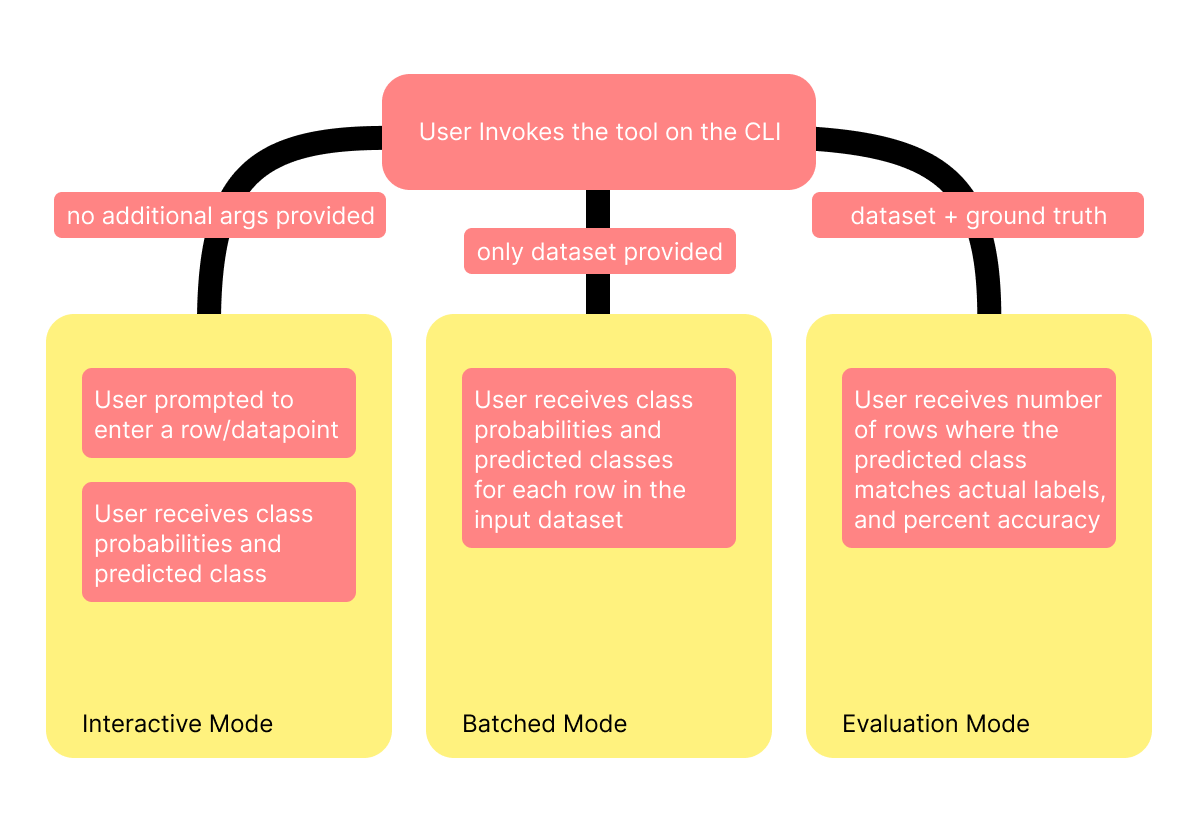
\includegraphics[width = \textwidth]{../images/UserFlow.png}
\end{center}

\subsubsection{Data Structures for Reconstruction}
In order to represent our loaded model architecture in memory, we define the following data structure in \verb|Lib.hs|:
\begin{lstlisting}
type Network = [Layer]

data Layer = Layer {
		weights :: Matrix R,
		biases :: Matrix R
	}
\end{lstlisting}
Here, we can see that the entire network is simply represented as a list of layers, with each layer storing its weights \& biases. The \verb|Matrix| type is imported from the hmatrix library, and \verb|R| is simply an alias for the double type.
\subsubsection{Parsing a model file}
With cereal, parsing the binary data format is quite uncomplicated. We have defined two functions:
\begin{lstlisting}
modelFileHead :: Get Network
modelFileHead = do
	layers <- getInt32le
	inputNeurons <- getInt32le
	modelFileCont (fromIntegral layers) (fromIntegral inputNeurons)

modelFileCont :: Int -> Int -> Get Network
modelFileCont left neuronsPrev = do
	if left == 0 then return []
	else do
		neurons <- getInt32le
		weightsList <- getDoubles (fromIntegral neurons * neuronsPrev)
		biasesList <- getDoubles (fromIntegral neurons)
		let weights = matrix neuronsPrev weightsList
			biases = matrix 1 biasesList
			layer = Layer weights biases
		rest <- modelFileCont (left - 1) (fromIntegral neurons)
		return $ layer:rest
	where
		getDoubles ::  Int -> Get [Double]
		getDoubles n = do
			if n == 0 then return []
			else do
				double <- getFloat64le
				rest <- getDoubles (n - 1)
				return $ double:rest	
\end{lstlisting}
The \verb|modelFileHead| function is responsible for parsing the "header" of the binary file, containing information about the number of layers and the number of neurons in the input layer. After this, we simply call the iterative \verb|modelFileCont|(ents) function, which iteratively parses and constructs the memory representation for each layer of the network.

\subsubsection{Challenges \& Mitigation}
Over the course of designing \& implementing the system, we ran into several pitfalls:
\begin{enumerate}
	\item \textbf{Migrating Libraries:}\\
	During the final stage of the project, we made several migrations to different libraries. Some of them were somewhat planned, for instance, the migration away from parsec, in favour of a binary file parsing library. However, even this one did not entirely go to plan. Initially, the idea was to swap to attoparsec, which would allow us to retain much of the structure of the initial parser. Unfortunately, attoparsec did not support parsing IEEE754 double precision floating point numbers out of the box, and would require us to implement our own conversion from its bitfields to the haskell type. As such, we decided to look further, finding the cereal library, which perfectly fit our needs.\bigskip

	While this migration went off relatively smoothly, besides the wasted time, some were more challenging. In the initial prototype we were naively using the Haskell standard matrix \& vector libraries. However, upon completing our literature survey, we realised that this was unacceptably slow compared to its alternatives, leading to us migrating to hmatrix, which in addition to requiring a rewrite of the entire inference module, also had some larger complications:

	\item \textbf{LAPack \& Blas}\\
	hmatrix owes most of its speed gains to it essentially being a wrapper for the industry standard numerical linear algebra packages, LAPack \& Blas, which are written in C. While the speed advantage this interoperation provides is great, it also brings with it a few challenges related to dependency management. Once we had rewritten the inference module for the new hmatrix backend, we realised that our project no longer compiled, owing to it missing these dependencies.\bigskip

	Trying to satisfy these dependencies led us down a small rabbithole, due to only finding very old and unreliable answers online, which was eventually resolved by a simple look into the Haskell Tool Stack documentation, which revealed that, on windows, it maintains its own MSYS2 environment. After installing LAPack \& Blas onto this environment, these issues were resolved, but not without taking away a lot of time from the development of the project.

	\item \textbf{Initial Benchmarks}\\
	In a later section, we talk about our benchmarks, and how they are less than satisfactory. However, in our initial benchmarks, even after the migration to hmatrix, we observed far worse results. After a bit of sleuthing, the culprit was narrowed down to an unsuspecting line of code:
	\begin{lstlisting}
col = (toColumns mat) !! colIdx
	\end{lstlisting}
	Put simply, this converts the matrix \verb|mat| into a list of column vectors, and then indexes that list to find the column at \verb|colIdx|. Of course, the problem we overlooked is that indexing raw lists in O(n) in Haskell, leading to bad outcomes. After discovering the column extraction operator in hmatrix, we simplified this line to:
	\begin{lstlisting}
col = flatten $ mat ? [colIdx - 1]
	\end{lstlisting}
	Which immediately led to an appreciable speedup of 4x. This is a testament to how, when interop is used to speed up computation, performance issues can often be invisiblised and easy to miss.
\end{enumerate}

\section{Results \& Discussion}
\subsection{Example Runs}
{
	\begin{center}
		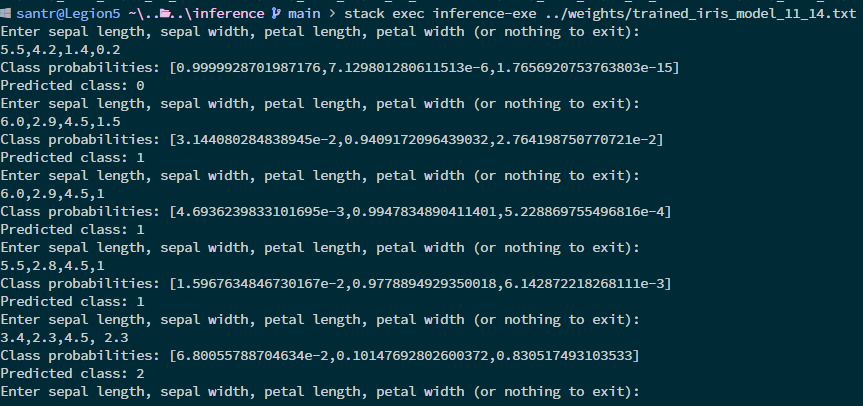
\includegraphics[width=\textwidth]{../images/examples.png}
	\end{center}
	\begin{center}
		Interactive Mode
	\end{center}
	\begin{center}
		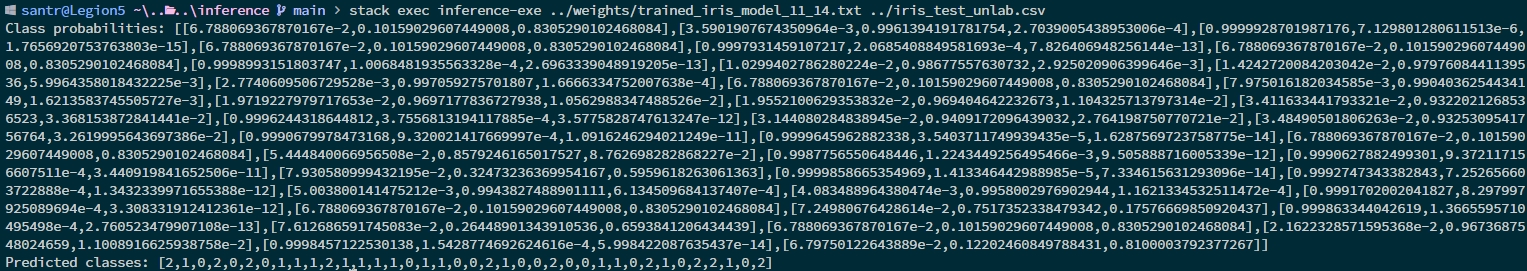
\includegraphics[width=\textwidth]{../images/examplebatch.png}
	\end{center}
	\begin{center}
		Batched Mode
	\end{center}
	\begin{center}
		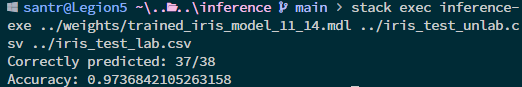
\includegraphics[width=\textwidth]{../images/exampleeval.png}
	\end{center}
	\begin{center}
		Evaluation Mode
	\end{center}
}

\begin{figure}[H]
	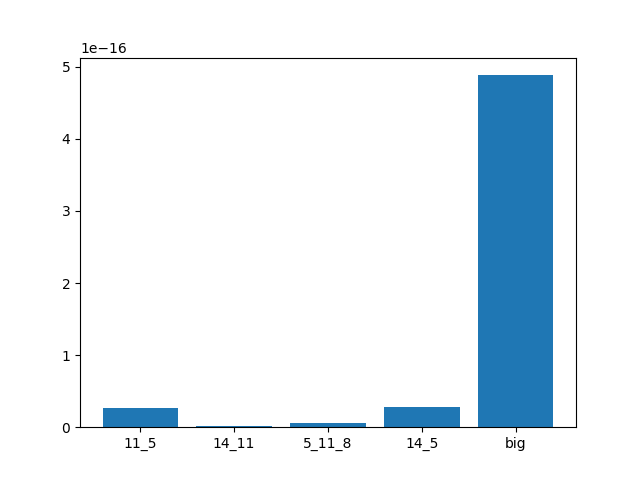
\includegraphics[width=\textwidth]{../images/mse.png}
	\caption{\centering \label{fig:3}the mean square error between the output activations observed in batch inference using sklearn and our system, on a variety of network shapes. The "big" network shape here refers to a 12-layer network}
\end{figure}
\subsection{Testing Outcomes}
During our end-to-end testing, as mentioned earlier in section \ref{sec:8.2.2}, we compare the output activations after batch inference from sklearn and our implementation. We run the inference on a batch of 20150 datapoints which we generate from the original testing set (sampling from the distribution of features in the original set). Figure \ref{fig:3} summarises our findings, displaying that the deviations observed are of the order of $10^{-32}$ to $10^{-30}$ in the extreme case, which are extremely minute and can be chalked up to floating point truncation or rounding errors that occur while reading the output of the inference module in the end-to-end testing script.

\subsection{Profiling Outcomes}
\begin{figure}
	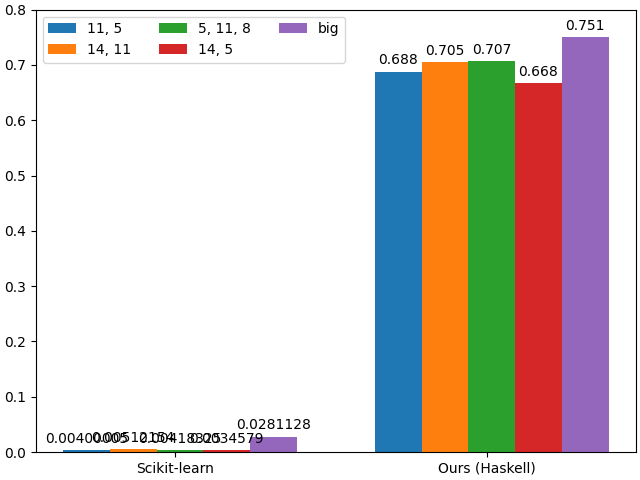
\includegraphics[width=\textwidth]{../images/benchmark.png}
	\caption{\centering \label{fig:4}a comparison of the run times of batch inference (50150 samples) with sklearn vs our implementation, for a variety of network shapes. The "big" network shape here refers to a 12-layer network}
\end{figure}
For profiling our implementation, we consider a variety of network shapes, and run batch inference on a generated dataset of size 20150. For each network shape, we run the inference 10 times, and report the average runtime in seconds. The comparison can be seen in Figure \ref{fig:4}.\bigskip

From the chart, it is apparent that despite us taking care to optimise our system, it fails to attain our profiling baseline (sklearn). In most cases, sklearn achieves a speedup of over $10$ when compared to our implementation. A quantification of how much of this disparity is an artifact of our relative inexperience with haskell vs an effect of the underlying language implementation requires further study.

\subsection{Limitations}
\begin{itemize}
	\item The command-line interface, while designed for usability, still may serve as a barrier for the most technically-challenged individuals
	\item Requires the weights to be in a particular format
	\item Class labels aren't currently considered, which hinders readability
	\item The system's performance, while optimised, fails to compete with sklearn's.
\end{itemize}

\section{Conclusions}
We have built a successful baseline inference package using haskell, though it is clear that it is far from complete. Besides lacking many configuration options and flexibility, it also fails to achieve the performance one would expect from a more standard package implemented in python with something like sklearn. Nonetheless, we have developed an accurate and acceptably performant system for inferencing feed-forward network classifiers.\bigskip

Further, we have expanded the scope of the project from the intial problem statement to provide a more general solution than was expected. In doing so, we have also provided a partial solution to the black-boxing problem discussed in section \ref{sec:3.1}.\bigskip

Finally, we were able to propose a specialised format for serializing trained feed-forward classifiers, which is space effective and utilises our understanding of the network architecture to achieve this optimisation.

\section{Extensions \& Future Work}
\begin{itemize}
	\item Infer the format of the weights file based on a few well-known formats (.pkl, .pth, .safetensors), instead of only working for our custom format. This requires more than just looking at the extension, as we have to further infer where the weights and biases of each layer lie based on the keys in the file. 
	\item The inference performance should be inspected more deeply and optimised accordingly.
	\item Currently, we have not performed any profiling on the parser, which is a core component of the entire system.
	\item A graphical user interface could greatly enhance the program's usability.
	\item Model input space could be extended to accept more architectures, such as support-vector machines or decision trees.
\end{itemize}

\section{References}
\begin{enumerate}
	\item \href{https://github.com/Magalame/fastest-matrices}{Haskell Linear Algebra Libraries Benchmark}
	\item \href{https://hoogle.haskell.org/}{Hoogle: Haskell Documentation Search Engine}
	\item \href{https://docs.haskellstack.org/}{Haskell Tool Stack Documentation}
	\item \href{https://hackage.haskell.org/}{Hackage: Haskell Package Registry}
	\item \href{https://wiki.haskell.org/}{Haskell Wiki}
	\item \href{https://book.realworldhaskell.org/}{Real World Haskell: An Introductory Book on Haskell}
\end{enumerate}

\end{document}

